\section{External interface requirements}
\label{sec:external_interface_requirements}

To be able to fulfill all of the requirements specified in section 3 some additional requirements for the WOMS has to be specified. These requirements are the \textbf{External interface requirements}, the requirements that specify how the WOMS will interact with other systems and users.  These requirements are separated into 3 different categories, depending on what they describe, \textbf{Software interface requirements}, \textbf{Communications interfaces requirements} and \textbf{Hardware interfaces requirements}. A more in detail description of each of the interfaces are described in their own subchapter, but the main focus can be seen as \textbf{Software interface requirements} is what information will be transmitted, \textbf{Communications interfaces requirements} is what type technical interface the communication will be on and \textbf{Hardware interfaces requirements} will be the hardware the WOMS comes in contact with. 

The requirements in this section is elicited from the Appendix A document \cite{A}, as well as interviews with the IS/IT-department. To get a greater understanding of how the WOMS will, technically, fit in the current ACME IT environment an overview of the communications are present in figure \ref{fig:external_interfaces}


\begin{figure}[H]
	\centering
	\setlength\fboxsep{7pt}
	\setlength\fboxrule{0.5pt}
	\fbox{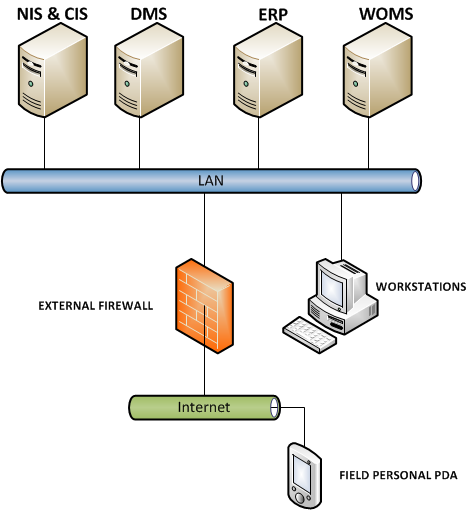
\includegraphics[scale = 0.8]{images/external_interfaces.png}}
	\caption{The external interfaces of the ACME network}
	\label{fig:external_interfaces}                      	
\end{figure}

All of the requirements in this section will be prioritized according to the MosCoW scheme, in the same way as the requirements in section \ref{sec:functional_requirements}.	

NOTE: No requirements on needed changes for other parts of the IT-system are listed here, only requirements that directly affect that WOMS are specified. I.e. there are no requirements on that the PDA needs to be able to connect to the LAN, see fig. \ref{fig:external_interfaces}, only requirements on how the PDA interacts with the WOMS while it's on the LAN.

\subsection{Software interfaces}
\label{sub:software_interfaces}

\textbf{Software interfaces} focuses on the connection the new WOMS will have with other system in the IT environment. Even though figure \ref{fig:external_interfaces} states that the WOMS will act like any other server in the network, the integration between WOMS and the current systems are far greater than the integration between the current systems.  In table \ref{table:software_interfaces} the software interfaces requirements that are needed are listed.

\begin{center}
\begin{longtable}{|l|p{4cm}|p{4cm}|l|l|}
\caption{Software interface requirements}
\label{table:software_interfaces}\\
\hline
\textbf{ID}& \textbf{Description} & \textbf{Comment} & \textbf{Priority} & \textbf{Dependencies}\\
\hline
\endfirsthead

\multicolumn{5}{c}%
{\tablename\ \thetable\ -- \textit{Continued from previous page}} \\
\hline
\textbf{ID}& \textbf{Description} & \textbf{Comment} & \textbf{Priority} & \textbf{Dependencies} \\
\hline
\endhead

\hline \multicolumn{5}{r}{\textit{Continued on next page}} \\
\endfoot

\hline
\endlastfoot

\hline

ERI-SI-1& The WOMS shall access the ERP to read any data & & & \\
\hline
ERI-SI-2& The WOMS shall access the ERP to update any data & & & \\
\hline
ERI-SI-3& The WOMS shall access the ERP to delete any data & & & \\
\hline
ERI-SI-4& The WOMS shall access the NIS to read any data & & & \\
\hline
ERI-SI-5& The WOMS shall access the NIS  to modify any data & & & \\
\hline
ERI-SI-6& The WOMS shall access the NIS  to delete any data & & & \\
\hline

\end{longtable}
\end{center}

\subsection{Communication interfaces}
\label{sub:communication_interfaces}

The current interaction of the systems are based on Ethernet connections, this will therefore be the main way the system connects with other systems in the network. Listed in table \ref{table:communication_interfaces} are all the requirements on the communication interfaces.

\begin{center}
\begin{longtable}{|l|p{4cm}|p{4cm}|l|l|}
\caption{Communication interface requirements}
\label{table:communication_interfaces}\\
\hline
\textbf{ID}& \textbf{Description} & \textbf{Comment} & \textbf{Priority} & \textbf{Dependencies}\\
\hline
\endfirsthead

\multicolumn{5}{c}%
{\tablename\ \thetable\ -- \textit{Continued from previous page}} \\
\hline
\textbf{ID}& \textbf{Description} & \textbf{Comment} & \textbf{Priority} & \textbf{Dependencies} \\
\hline
\endhead

\hline \multicolumn{5}{r}{\textit{Continued on next page}} \\
\endfoot

\hline
\endlastfoot

ERI-CI-1& All communication on the LAN, with the WOMS, shall be on Ethernet. & & Must & \\
\hline
ERI-CI-2& The WOMS only access way to units outside the ACME LAN is through the firewall, via Ethernet. & Units, will be, but are not limited to, PDAs & Must & \\
\hline

\end{longtable}
\end{center}


\subsection{Hardware interfaces}
\label{sub:hardwar_interfaces}

A \textbf{Hardware interfaces} requirement is a requirement specifying what kind of other hardware that will communicate with the WOMS. The WOMS will need to be accessible from both internal workstations, as well as external PDAs, see fig. \ref{fig:functional_requirements}. To achieve this there are some hardware interfaces requirements that needs to be fulfilled:

\begin{center}
\begin{longtable}{|l|p{4cm}|p{4cm}|l|l|}
\caption{Hardware interface requirements}
\label{table:communication_interfaces}\\
\hline
\textbf{ID}& \textbf{Description} & \textbf{Comment} & \textbf{Priority} & \textbf{Dependencies}\\
\hline
\endfirsthead

\multicolumn{5}{c}%
{\tablename\ \thetable\ -- \textit{Continued from previous page}} \\
\hline
\textbf{ID}& \textbf{Description} & \textbf{Comment} & \textbf{Priority} & \textbf{Dependencies} \\
\hline
\endhead

\hline \multicolumn{5}{r}{\textit{Continued on next page}} \\
\endfoot

\hline
\endlastfoot

ERI-HI-1& The WOMS shall exchange data with the all servers on the LAN. & Servers are, the NIS \& CIS server, the DMS server and the ERP server. & Must & \\
\hline
ERI-CI-2& The WOMS shall be accessible from the Field Personal PDAs. & & Must & \\
\hline

\end{longtable}
\end{center} 

